\documentclass[a4paper]{article}
\usepackage[margin=1in]{geometry}

\usepackage[english]{babel}
\usepackage[utf8]{inputenc}
\usepackage{amsmath}
\usepackage{amsfonts}
\usepackage{natbib}
\usepackage{graphicx}
\usepackage[auth-sc,affil-sl]{authblk}
\usepackage[table]{xcolor}

\usepackage[colorinlistoftodos]{todonotes}
\usepackage{hyperref}
\usepackage{enumitem}
\usepackage{pdfpages}
\usepackage{framed}
\usepackage{float}
\usepackage[tableposition=top]{caption}



\addto{\captionsenglish}{\renewcommand{\abstractname}{Executive Summary}}

\title{Usability Test Report of CP's Website\\ (Proposal)}
\author[1]{Tested by: Luís  Cruz}
\affil[1]{MAP-i\\ Joint Doctoral Programme in Computer Science}
\date{Tested: January 20, 2014}

\begin{document}
\maketitle

Common Industry Format for Usability Test Report v1.1

Date prepared: January 27, 2014

Prepared by: Luís Cruz (luiscruz@fe.up.pt)

\begin{abstract}
	
	This document intends to report the usability test for the website \emph{CP.pt} in the scope of the unit course of Interactive Computing Systems(ICS) of the MAP-i doctoral programme. The usability test was conducted by inviting two potential users to accomplish four tasks, using the \emph{think-aloud} technique, while using some behavior analysis/acquisition methods. The participant's activity was recorded through screen and audio cast, and the moderator observed the participant by taking notes in the provided Data Logging Form. After each task, a short interview had place, and after the whole test, users were asked to answer a customized 30 questions survey, as well as the System Usability Scale (SUS) questionnaire.

The recruited participants were screened in order to focus on college students that need to travel to their universities. 

With this study some usability issues were spotted, but the results were satisfactory. All the users were able to complete all the tasks, and despite some inefficiencies in some steps, the completion rate efficiency was $38\%/min$.
The overall website satisfaction of the users was perceived as \emph{good}, assessed using the SUS scale that scored 60 out of 100. The feedback obtained from users through the interviews helped to find some issues in the user interface that need special attention.
\end{abstract}

\section{Introduction}
\subsection{Product Description}

CP.pt is the official website of emph{CP - Comboios de Portugal, E.P.E}, the public portuguese company responsible for rendering national and international passenger rail services.

CP customers vary according to the service provided. Many college students, workers and pensioners use the regional and urban services for small and medium distances. Long distance services are more used by college students that are away from home, tourists, and executive workers. Unfortunately, no official document stating the segmentation of the CP.pt website's users was found.

It is noticeable that CP services have a lot more passengers during school time, which means that students are an important segment of CP's customers. Besides, most of the students have good experience with the WEB, so the CP.pt website is expected to be a great tool to them. Therefore, this usability evaluation will focus in the segment of college students, which might be portuguese citizens as well as foreigners that study or want to study in Portugal and are able to speak English.

Many scenarios can apply for the use of the website by students. Some times they leave the classes earlier and need a way of quickly check if there are other alternative trains that can take them home earlier. Also sometimes there is no direct train to their destination, so they have to catch another in the the middle of the travelling. Another scenario is when the weekend is over and the student has to buy his/her ticket from home to his/her university city. Buying it from the website is more convenient since the student can avoid wasting time in the ticket lines and can grant a seat for his/her trip.

From the features implemented in the website, the following were tested:
\begin{itemize}
  \item Choose between Portuguese or English versions
  \item Check timetables for a trip.
  \item Buy fast train tickets, being the features that were tested.
\end{itemize}


\subsection{Test Objectives}

The aim of the test was to validate the usability of the main features of the CP.pt --- finding the most suitable train and buying tickets. It is important that these tasks are easy to learn.

Representative users were asked to complete some tasks, measures were taken of effectiveness, efficiency and satisfaction, and some notes about the users' opinion were taken in order to have ideas for some improvements that can be made.

\section{Method}

\subsection{Participants}

This test had 2 participants, both college students with ages between 21 and 26 years old. Regarding the small size of the sample, 100\% of the participants were female.

They are intermediate level users, that frequently use WEB applications and already have experience in other transportation company's websites (e.g., \emph{Ryanair}). This characteristics are expected in the population of college students, except for the gender that should be in equal portion, and the ages that could be more representative --- students enter to college in ages starting from 17 years old.

\subsection{Context of Product Use in The Test}
\subsubsection{Tasks}
\label{sec:tasks}
The tasks that the participant has to accomplish are the following:

\begin{enumerate}
  \item Select the English Version of the application.
  \item Find the schedule for a trip from Braga to Aveiro.
  \item Find a cheap trip from Braga to Aveiro.
  \item Buy a ticket from Braga to Porto.
\end{enumerate}

These tasks are described in more detail in the \emph{Usability Test Plan}, available in the appendix~\ref{sec:usabilityTestPlan}. For each task, all the steps were defined in order to describe how the task can be efficiently accomplished.

These tasks were selected with the criteria of being features that are expected to be of the most important use. Every transportation website has these features and add great value to the customers, so it is important that \emph{CP.pt} meets the users needs.

All the completion and performance criteria are also described in the Usability Test Plan (see appendix~\ref{sec:usabilityTestPlan}).

\subsubsection{Test Facility}

The test was made in a study room at the faculty. The moderator is sitting next to the participant in order to make the observation and query and give assistance. The screen and audio were recorded using the tool QuickTime Player 10.3 which is invisible to the user and does not affect the user experience.

\subsubsection{Participant’s Computing Environment}

According to~\citep{satya2013resolution}, the most common resolution used in WEB is $1366\times 768$. In this experiment a 13 inches RGB screen with approximately the same resolution was used: $1440\times 990$. For interaction with the application the participant used an Apple laptop keyboard, and an Apple Magic mouse. Some other devices were available if the user didn't feel comfortable with these devices, however, they were not used.

The browser Safari 7.0.1 with default settings was used with an internet connection which had an average download and upload speeds of $4 Mbit/s$ and $1Mbit/s$, respectively.


\subsubsection{Test Administrator Tools}

A \emph{Data Logging Form} (see~\ref{sec:dataLoggingForm}) was designed providing the moderator with a tool to record some notes about each task of each participant. The form has some fields for a few variables and a space to take some notes for the post-task interview.

All the task information is provided in the \emph{Usability Test Plan}, available in the appendix~\ref{sec:usabilityTestPlan}, defining a script about how the moderator should conduct the experiment is provided. All the steps that are necessary to finish a task are clearly described as well as some guidelines with the important questions for the post-task interview.

After the test, the participants were asked to answer a post-test questionnaire based on~\citep{lawton2004wai_ut} provided in appendix~\ref{sec:postTestQuestionnaire} and the SUS questionnaire available in the literature~\citep{brooke1996sus}.

As it was already mentioned, during the experiments, the screen and voice were recorded using the tool QuickTime Player 10.3.

\subsection{Experimental Design}

Two college students were tested. For each of the four tasks, described above, the completeness, number of assistances, number of steps made differently, back button hits, number of errors, and the duration of the task were recorded. The completion rate, unassisted completion rate, and completion rate efficiency were calculated.

\subsubsection{Procedure}

The participants were informed that the usability of CP's website was being tested, to find out whether it met the needs of users. They were told that it was not a test of their abilities. They were asked to sign a consent form.

Participants were given introductory instructions. The evaluator reset the state of the computer before each task, and provided instructions for the next task. 

The participant could ask for assistance and make questions whenever they find necessary, in order clarify any part of the task. All assistances were logged by the moderator. Also there was no time limit for the task completions, but if the moderator feels that the participant is stuck in some part, he was allowed to give some hints if properly logged.

After each task the moderator conducted a small interview trying to answer some crucial questions provided in the Usability Test Plan (see appendix~\ref{sec:usabilityTestPlan}).

In the end of the test, a post-test questionnaire based on~\citep{lawton2004wai_ut} was given to the participants (available in appendix~\ref{sec:postTestQuestionnaire}).
This questionnaire has a Likert response format in a scale from 1 to 5, and intends to provide some insights about the way the design should be changed to make it more suitable to the user.

In addition to this questionnaire, the users are asked to fill the SUS questionnaire~\citep{brooke1996sus}.

The participants were non remunerated voluntaries and during each test session only the moderator and a participant were present.

\subsubsection{Participant General Instructions}

The instructions were given personally by the moderator to each participant. The test session proceeds by having only one user in the room with a moderator. Whenever the user needed help he/she could simply ask for help.

The participant was asked to use the \textit{think-aloud} technique, describing every step he/she makes during the tasks.

\subsubsection{Participant Task Instructions}
Before starting each task the moderator explained what it was expected to accomplish in the following task. The task instructions are very simple, being described in a short sentence, as stated in section~\ref{sec:tasks}.

\subsection{Usability Metrics}
\label{sec:usability_metrics}

\subsubsection{Effectiveness}
For measuring effectiveness the following measures were considered:

\begin{description}
    
 \item[Completion Rate] the percentage of participants that correctly finished each task.
 \item[Unassisted Completion Rate] the percentage of participants that correctly finished each task without assistance.
 \item[Number of Assistances] The average of assurances given in each task.
 \item[Number of steps made differently] number of steps that the participants made differently to the ones described in the test plan.
 \item[Back Button hits] The average of times the user hit the Back Button in the browser.
 \item[Errors] The number of times a user had to repeat parts of the task.

\end{description} 
 
 \subsubsection{Efficiency}
 Efficiency was accessed by measuring the following parameters:
\begin{description}  
  \item[Task time] The average time the users took to correctly complete each task.
 \item[Completion rate efficiency] mean completion rate/mean task time (in minutes).
\end{description} 
 
\subsubsection{Satisfaction}
Satisfaction is a subjective measure that correlates with the user's motivation to use a product. The standardized instrument \textit{System Usability Scale} (SUS) provides a 10 item questionnaire with five-scale responses that can be converted into a score~\citep{brooke1996sus}. After the test the users answered this questionnaire. 
 
Also a post-test questionnaire based on~\citep{lawton2004wai_ut} was given to the participants (available in appendix~\ref{sec:postTestQuestionnaire}).
Although this questionnaire does not provide a metric result, it is an useful tool to obtain user's feedback.
 
 
 \section{Results}
 \subsection{Data Analysis}
 \subsubsection{Data Scoring}
 The method by which the data collected were scored should be described in sufficient detail to allow replication of the data scoring methods by another organization if the test is repeated. Particular items that should be addressed include the exclusion of outliers, categorization of error data, and criteria for scoring assisted or unassisted completion.
 
\subsubsection{Data Reduction}

  Based on the data acquired in each task, combined results were derived with mean results for effectiveness and efficiency metrics per participant and per task.
  
\subsection{Presentation of the Results}
   Effectiveness, Efficiency and Satisfaction results must always be reported

\subsubsection{Performance Results}
 Performance results refer to the results achieved with effectiveness and efficiency metrics, described above in section~\ref{sec:usability_metrics}.
 \paragraph{Task 1} This task was extremely easy for all participants. Every user completed the task correctly with no assistances and no inefficiency. The results observed in task 1 are reported in table~\ref{table:results_task_1}. \textbf{Completion rate efficiency} is $13\%/s$. Although this was a trivial task, it was important for the user to get familiar with the test setup and procedure.
 
 \begin{table}[H]
\begin{center}
  \caption{Results observed in \textbf{task 1}.}

  \label{table:results_task_1}
\begin{tabular}{ c | c | c | c | c | c | c}

\hline
Participant ID       &
Completion &
\parbox{5em}{\centering Number of Assistances} &
\parbox{8em}{\centering Number of steps made differently } &
\parbox{6em}{\centering Back Button hits}  & 
Errors  &
Time\\
\hline
1                    &  1                  &  0                    &  0                &  0        &  0   & 0'08''\\   
2                    &  1                  &  0                    &  0                &  0        &  0   & 0'08''\\ 
\hline                                                                                                    
Mean                 &  1                  &  0                    &  0                &  0        & 0    & 0'08'' \\   
Std Dev              &  0.0                &  0.0                  &  0.0              &  0.0      & 0.0  & 0'00''  \\   
Min                  &  1                  &  0                    &  0                &  0        & 0    & 0'08''\\   
Max                  &  1                  &  0                    &  0                &  0        & 0    & 0'08''\\   
\hline

\end{tabular}
\end{center}
\end{table}
% -------------------------- %
 
\paragraph{Task 2} The results observed in task 2 are reported in table~\ref{table:results_task_2}. \textbf{Completion rate efficiency} is $38\%/min$.

 \begin{table}[H]
\begin{center}
\caption{Results observed in \textbf{task 2}.}
\label{table:results_task_2}
\begin{tabular}{ c | c | c | c | c | c | c}

 \hline
Participant ID       & 
Completeness  &
\parbox{5em}{\centering Number of Assistances} &
\parbox{8em}{\centering Number of steps made differently } &
\parbox{6em}{\centering Back Button hits}  &
Errors &
Time\\
\hline
1                    &  1                  &  1                    &  1                &  2        &  3    & 3'50''\\   
2                    &  1                  &  0                    &  2                &  1        &  0    & 1'25''\\   
\hline                                                                                                     
Mean                 &  1                  &  0.5                  &  1.5              &  1.5      & 1.5   & 2'38''\\   
Std Dev              &  0.0                &  0.5                  &  0.5              &  0.5      &  1.5  & 1'13'' \\   
Min                  &  1                  &  0                    &  1                &  1        &  0    & 1'25''\\   
Max                  &  1                  &  1                    &  2                &  2        & 3     & 3'50''\\   
\hline                                                                                                     

\end{tabular}
\end{center}
\end{table}
% -------------------------- %
\paragraph{Task 3} The results observed in task 3 are reported in table~\ref{table:results_task_3}. \textbf{Completion rate efficiency} is $87\%/min$. Although the task was very similar to the previous one, we can see that, in average, users needed less time to accomplish it (mean time was 1 minute and 9 seconds, which is a considerable decrease). This might be an indicator that the system is a lot easier for second time visitors.

 \begin{table}[H]
\caption{Results observed in \textbf{task 3}.}
\begin{center}
\begin{tabular}{ c | c | c | c | c | c | c}

 \hline
Participant ID       &
Completeness  &
\parbox{5em}{\centering Number of Assistances} &
\parbox{8em}{\centering Number of steps made differently } &
\parbox{6em}{\centering Back Button hits} &
Errors  &
Time\\
\hline
1                    &  1                  &  0                    &  0                &  0        & 0    & 0'50'' \\   
2                    &  1                  &  0                    &  0                &  0        & 0    & 1'28'' \\   
\hline                                                                                                    
Mean                 &  1                  &  0                    &  0                &  0        & 0    & 1'09'' \\   
Std Dev              &  0.0                &  0.0                  &  0.0              &  0.0      & 0.0  & 0'19'' \\   
Min                  &  1                  &  0                    &  0                &  0        & 0    & 0'50''\\   
Max                  &  1                  &  0                    &  0                &  0        & 0    & 1'28''\\   
\hline

\end{tabular}
\end{center}
\label{table:results_task_3}
\end{table}
% -------------------------- %

\paragraph{Task 4} The results observed in task 4 are reported in table~\ref{table:results_task_4}. \textbf{Completion rate efficiency} is $16\%/min$. Since this task was more complex, it took a lot more than the others: in average, users took 6 minutes and 27 seconds to complete. 

 \begin{table}[H]
   \caption{Results observed in \textbf{task 4}.}
   \label{table:results_task_4}
\begin{center}
\begin{tabular}{ c | c | c | c | c | c | c}

 \hline
Participant ID       &
Completeness  &
\parbox{5em}{\centering Number of Assistances} &
\parbox{8em}{\centering Number of steps made differently } &
\parbox{6em}{\centering Back Button hits}  &
Errors &
Time\\
\hline
1                    &  1                  &  3                    &  0                &  0        & 0    & 6'45'' \\   
2                    &  1                  &  0                    &  1                &  2        & 0    & 6'08''\\   
\hline                                                                                                    
Mean                 &  1                  &  1.5                  &  0.5              &  1        & 0    & 6'27''\\   
Std Dev              &  0.0                &  1.5                  &  0.5              &  1.0      & 0.0  & 0'19'' \\   
Min                  &  1                  &  0                    &  0                &  0        & 0    & 6'08''\\   
Max                  &  1                  &  3                    &  1                &  2        & 0    & 6'45''\\   
\hline

\end{tabular}
\end{center}
\end{table}
% -------------------------- %


% ------------------------------------------------ %
%                  COMBINED RESULTS                %
% ------------------------------------------------ %
\paragraph{Combined Results} The overall results of efficiency and effectiveness are combined in the table~\ref{table:combined_results}. It is possible to see that all users were able to finish all the tasks. These results suggest that some of the tested features are not very intuitive, since the back button was hit by users with an average of 2.5 times. Besides, 25\% of the experiment tasks were completed with assistance. The average time to complete is 2 minutes and 35 seconds, however, this measure is lowered by the fact that task 1 was really simple and took 8 seconds for the users to complete. In addition, the mean \textbf{completion rate efficiency} is $38\%/min$ --- ignoring the data from first task, this measure would decrease to $29\%/min$.

 \begin{table}[H]
\begin{center}
  \footnotesize
\caption{Combined Performance Results.}
\label{table:combined_results}
\begin{tabular}{ c | c | c | c | c | c | c | c }

 \hline
Participant ID       &
\parbox{5em}{\centering Completion Rate\\(\%)} &
\parbox{6em}{\centering Unassisted Completion Rate\\(\%)}  &
\parbox{4.5em}{\centering Number of Assistances} &
\parbox{8em}{\centering Number of steps made differently } &
\parbox{4em}{\centering Back Button hits}  &
Errors &
Time\\
\hline
1                    &  100       & 50          &  4                    &  1                &  2        & 3 & 2'53'' \\   
2                    &  100       & 100         &  0                    &  3                &  3        & 0 & 2'17''\\  
\hline 
Mean                 &  100       & 75          &  2                    &  2                &  2.5      & 1.5 & 2'35''\\   
Std Dev              &  0         & 25          &  2.0                  &  1.0              &  0.5      & 1.5 & 0'18''\\   
Min                  &  100       & 50          &  0                    &  1                &  2        & 0   & 2'17''\\   
Max                  &  100       & 100         &  4                    &  3                &  3        & 3   & 2'53''\\   
\hline

\end{tabular}
\end{center}
\end{table}
% -------------------------- %


 \subsubsection{Satisfaction Results}

\begin{table}[h!]
\caption{SUS results}
\label{table:sus}
\begin{center}
\begin{tabular}{c| c | c}
\hline
Participant ID & Total Score & SUS Score \\
\hline
1    &  25  & 62.5 \\
2    &  23  & 57.5  \\
\hline
Mean &  24   & 60.0\\
Min  &  23   & 57.5\\
Max  &  25   & 62.5\\
\hline
\end{tabular}
\end{center}
\end{table}

\begin{figure}[h] 
	\centering
	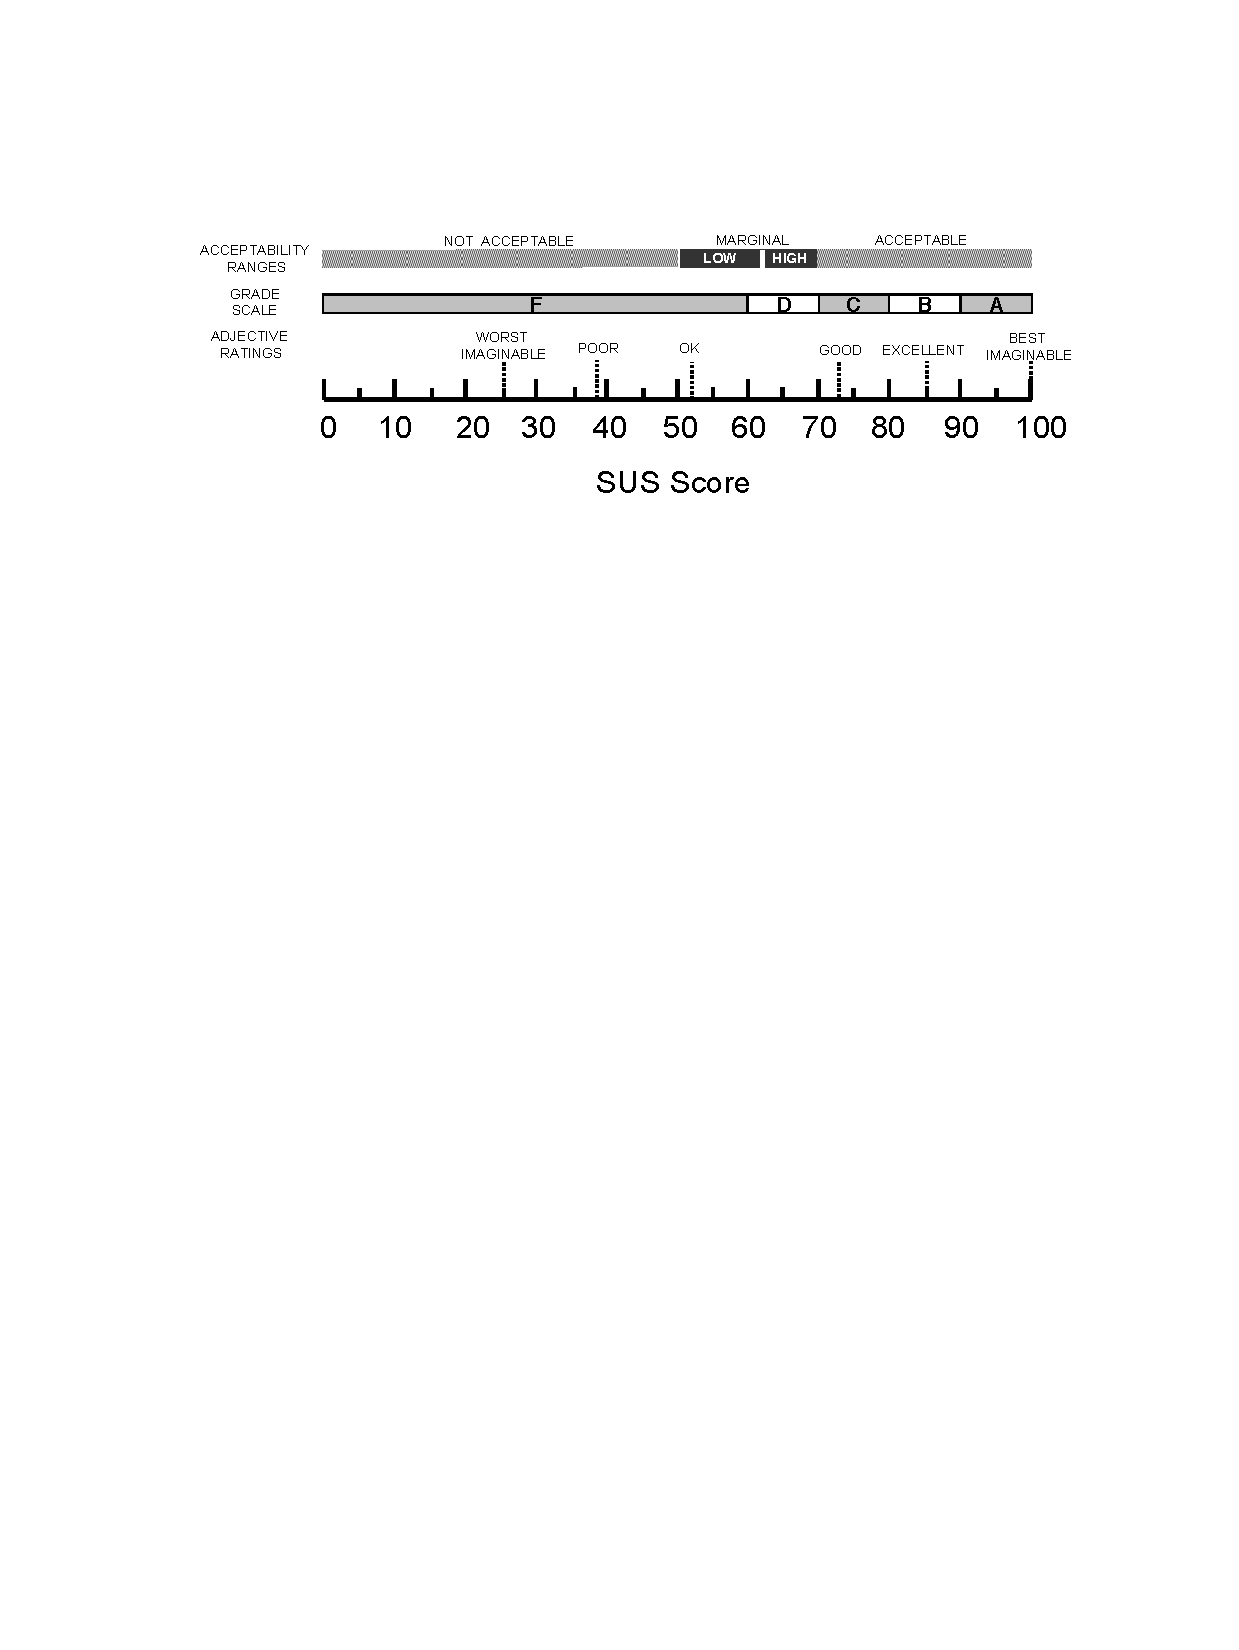
\includegraphics[width=0.8\textwidth]{figures/sus_qualititative_scale.pdf}
 	\caption{A comparison of the adjective ratings, acceptability scores, and school grading scales, in relation to the average SUS score. Source:~\citep{bangor2009determining}}
	\label{fig:sus}
\end{figure}

The mean SUS score achieved is 60 (out of 100). Using the \textit{Adjective Rating Scale} proposed by~\citet{bangor2009determining}, detailed in the figure~\ref{fig:sus}, the website was perceived by the participants as \textbf{good}.

\begin{table}[H]
\caption{Post-test questionnaire results}
\label{table:post-test_results}
\begin{center}
\footnotesize
\rowcolors{2}{black!10}{white}
\begin{tabular}{p{30em}| c | c | c}
\hline
\textbf{Question} & \textbf{User 1} & \textbf{User 2}  & \textbf{Mean} \\
\hline
1. The homepage is attractive                            &  2  & 4 & 3 \\
2. The overall site is attractive                        &  2  & 4 & 3  \\     
3. The site's graphics are pleasing                      &  3  & 4 & 3.5   \\
4. The site has a good balance of graphics versus text   &  3  & 4 & 3.5   \\
5. The colors used throughout the site are attractive    &  3  & 4 & 3.5   \\
6. The typography is attractive                          &  3  & 4 & 3.5   \\
7. The homepage’s content makes me want to explore the site further  & 3  &  3 & 3   \\
8. It is easy to find one’s way around the site                &  4  &  2 & 3  \\
9. You can get information quickly                             &  3  &  2 & 2.5  \\
\rowcolor{red!20}
10. It is fun to explore the site                              &  2  &  2 & 2  \\
\rowcolor{green!20}
11. It is easy to remember where to find things                &  4  &  4 & 4  \\
12. Information is layered effectively on different screens    &  3  &  4 & 3.5  \\
13. The homepage is attention-getting                          &  3  &  3 & 3  \\
14. Information is easy to read                                &  3  &  3 & 3  \\
15. Information is written in a style that suits me            &  3  &  4 & 3.5  \\
16. Screens have the right amount of information               &  2  &  4 & 3 \\
\rowcolor{green!20}
17. The site effectively communicates the company’s image      &  4  &  4 & 4  \\
\rowcolor{green!20}
18. Information is relevant                                    &  4  &  4 & 4  \\
19. The site is designed with me in mind                       &  3  &  3 & 3  \\
\rowcolor{green!20}
20. The site’s content interests me                            &  4  &  5 & 4.5  \\
\rowcolor{green!20}
21. The site’s content would keep me coming back               &  4  &  5 & 4.5  \\
22. The site has characteristics that make it especially appealing  &  3  & 3 & 3   \\
23. The site reflects progressive, leading edge design         &  2  &  3 & 2.5  \\
24. The site is exciting                                       &  2  &  3 & 2.5  \\
\rowcolor{red!20}
25. The site is well-suited to first-time visitors             &  2  &  1 & 1.5  \\
26. This site is well-suited to repeat visitors                 &  2  &  4 & 3  \\
27. The site has a clear purpose                               &  3  &  4 & 3.5  \\
28. It is always clear what to do next                         &  3  &  2 & 3.5  \\
29. It is clear how screen elements work                       &  2  &  5 & 3.5  \\
30. Mistakes are easy to correct                               &  4  &  1 & 2.5  \\
\hline
\end{tabular}
\end{center}
\end{table}

The results of the post-test questionnaire are presented in the table~\ref{table:post-test_results}. From all the answers the most relevant notions we get are that users agree that the website has relevant content that meets the users' needs and that the design of the website matches CP's image. However, they state that it is not well-suited for first-time visitors, and navigating through the website is not fun.


\subsection{Observation and Interview Results}

As mentioned earlier, after each task, a small interview was performed in order to get the most from user's opinion.
Besides, the moderator was standing next to the participant in order to find out the cause of some user's errors or inefficiencies. 
It allowed to spot some problems that can be solved in order to improve the website usability.

Some remarks made from the users was that the website is not well organized.

\paragraph{Task 1 - Select the English Version} Users clearly understood what they had to do, and recognized the british flag as a familiar icon for choosing the english version.

\paragraph{Task 2 - Find a train from Braga to Aveiro} During this task some usability problems were perceived. The ``Timetable and Prices'' form is not easy to find. Even experienced users made the mistake of using the NETTicket form which only provides trains for some services. Also, one user that is used to travel in the Urban service lines complained that train connections that take some time (e.g. 30 min) were not available, but when she travels usually prefers these ones for being cheaper. Also, there was some information that they found necessary to ask in the ticket office: discount prices and in which line do they have to switch in the middle of the the trip.

\paragraph{Task 3 - Find a cheap train from Braga to Aveiro} In this task, users complained about the timetable results table. They found annoying having to click in a link every time they want to check one train's price, and suggested to introduce some filters according to price, service line, etc.
 
\paragraph{Task 4 - Buy a ticket from Braga to Porto} The major difficulty was to select the seat, it was not intuitive, but after knowing how to use it they were able to complete the task with no problem. During the registration process, users didn't understand the form asking information about the most preferred lines. Furthermore, there is an important issue that should be fixed: when an unregistered users searches for a ticket and decides to buy it, the system redirects to the registration process; however, after registering, the user has to search again for the train, which is very inefficient and might be frustrating for the user.

\paragraph{} The screen and audio recording of the test including interviews is available at this usability project's website (url: \url{http://paginas.fe.up.pt/~luiscruz/cp_usability/}).

% ----------------------------------- %

%    APPENDIX+
\appendix

\section{Consent and Recording Release Form}
The present \emph{Consent and Recording Release Form} was adapted from a template available at \textit{Usability.gov} website\footnote{(url: \url{http://usability.gov})}.

\begin{oframed}
  \begin{center}
    \large \textsc{Consent and Recording Release Form}
  \end{center} 
I agree to participate in the study conducted and recorded by the MAP-i student Luís Cruz. 

I understand and consent to the use and release of the recording by Luís Cruz. I understand that the information and recording is for research purposes only and that my name and image will not be used for any other purpose. I relinquish any rights to the recording and understand the recording may be copied and used by Luís Cruz without further permission. 

I understand that participation in this usability study is voluntary and I agree to immediately raise any concerns or areas of discomfort during the session with the study administrator.

Please sign below to indicate that you have read and you understand the information on this form and that any questions you might have about the session have been answered. 

~

Date: \rule{2cm}{0.4pt} 

Please print your name: \hrulefill

Please sign your name: \hrulefill



Thank you!

Your participation is kindly appreciated.
\end{oframed}

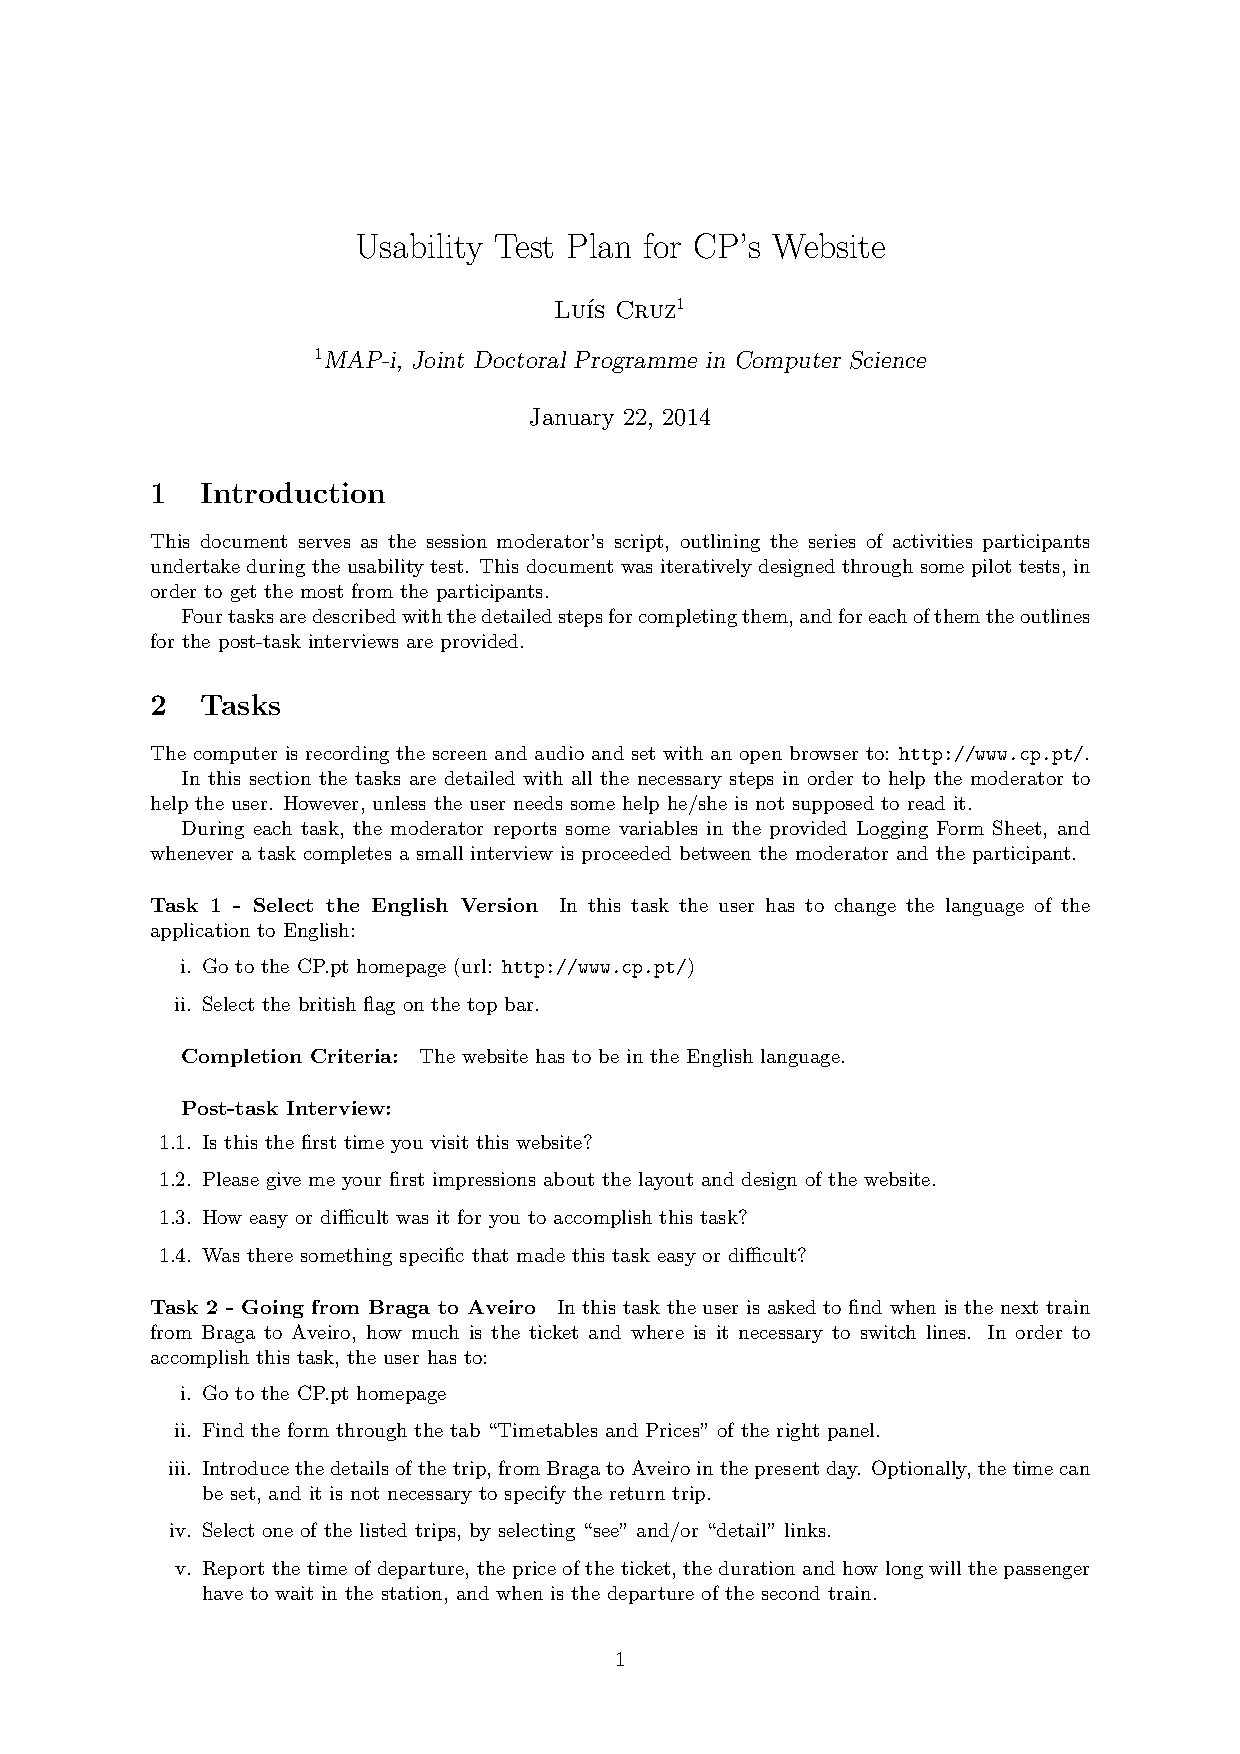
\includepdf[pagecommand=\section{Usability Test Plan}\label{sec:usabilityTestPlan}\thispagestyle{plain}{The plain original document can be accessed at \url{http://paginas.fe.up.pt/~luiscruz/cp_usability/}}, nup=2x2, pages=-, frame=true, scale=0.78, offset=0 -25]{../usabilityTestPlan/master.pdf}

% ------- DATA LOGGIN FORM -------- %

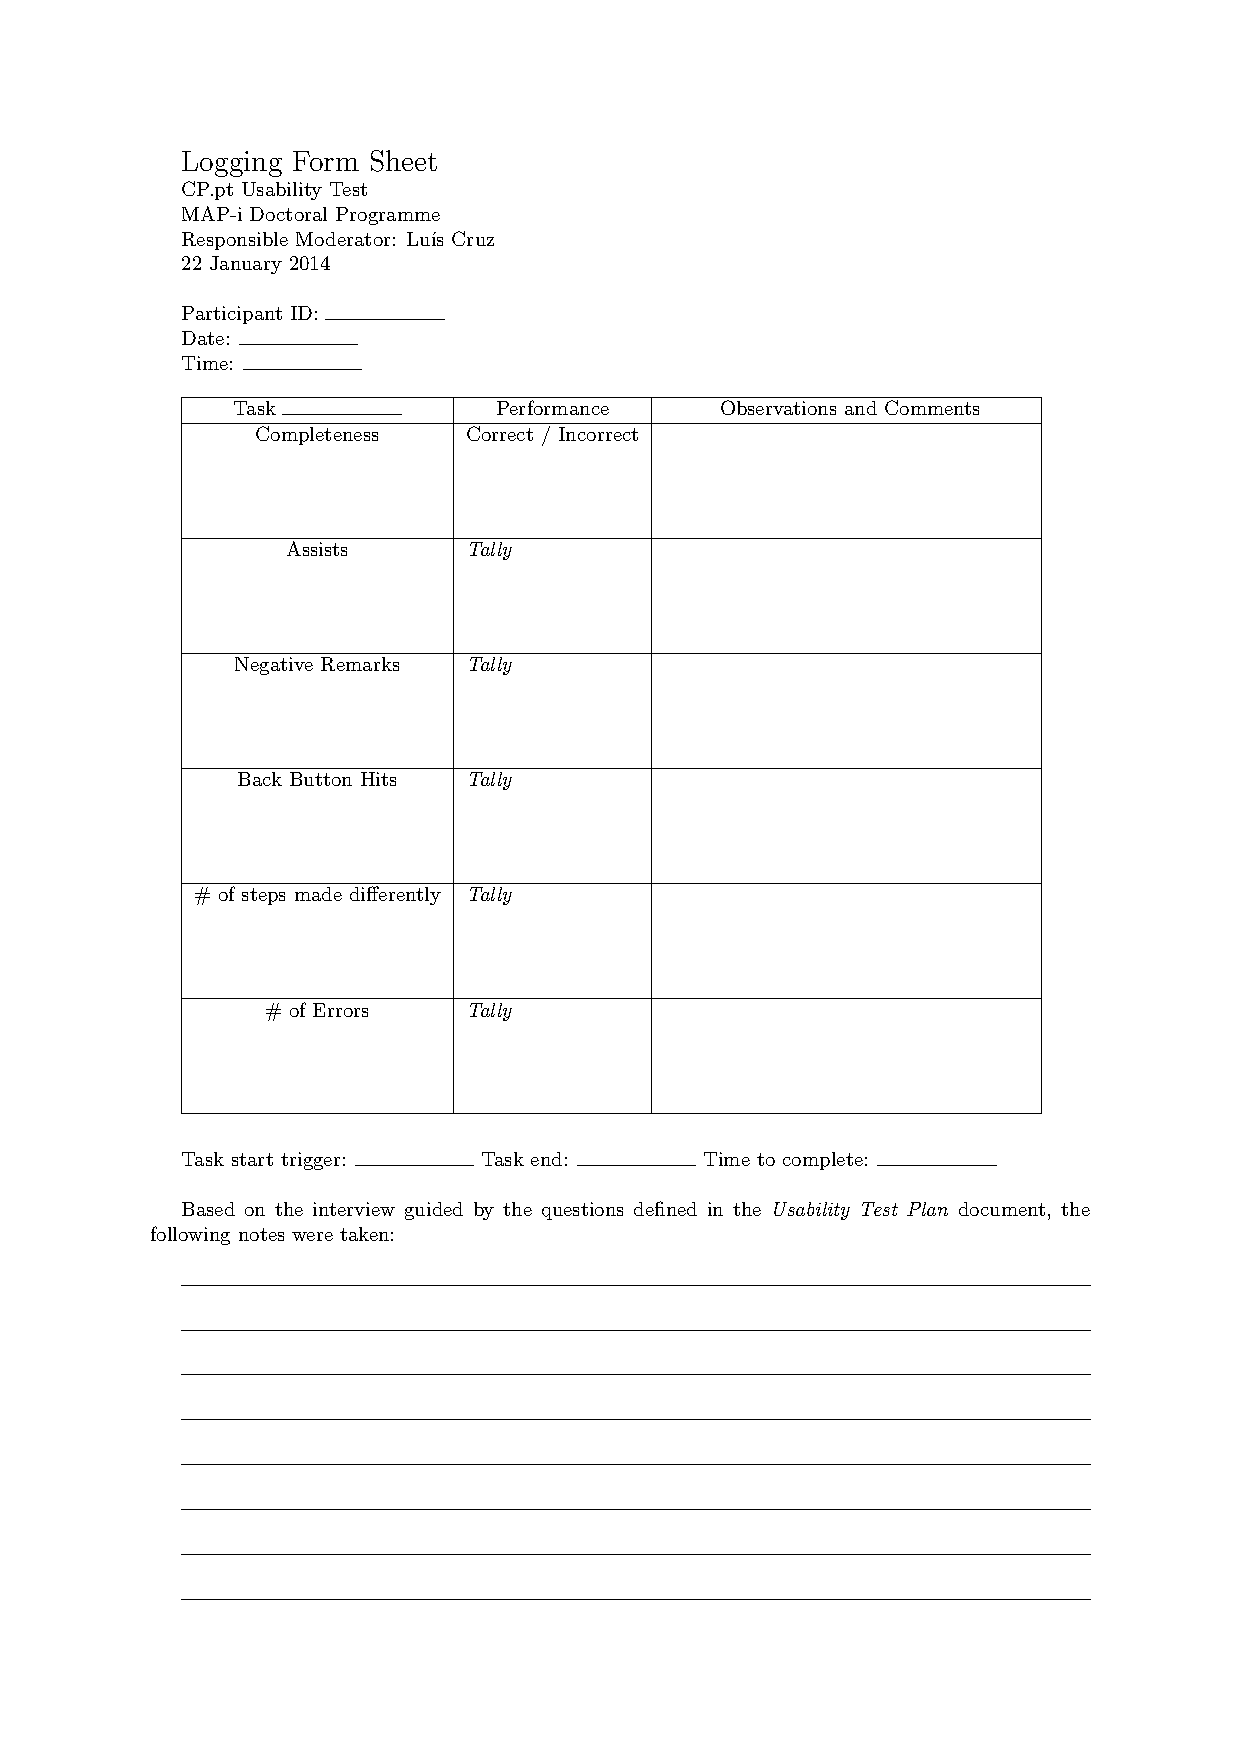
\includepdf[pagecommand=\section{Data Logging Form}\label{sec:dataLoggingForm}\thispagestyle{plain}{The moderator of the usability test observes the behavior of the participant while taking notes in the Data Logging Form. Each task needs one Data Logging Form.}, pages=-, frame=true, scale=0.75, offset=0 -25]{../dataLoggingForm/master.pdf}


% ---------------~o~--------------- %

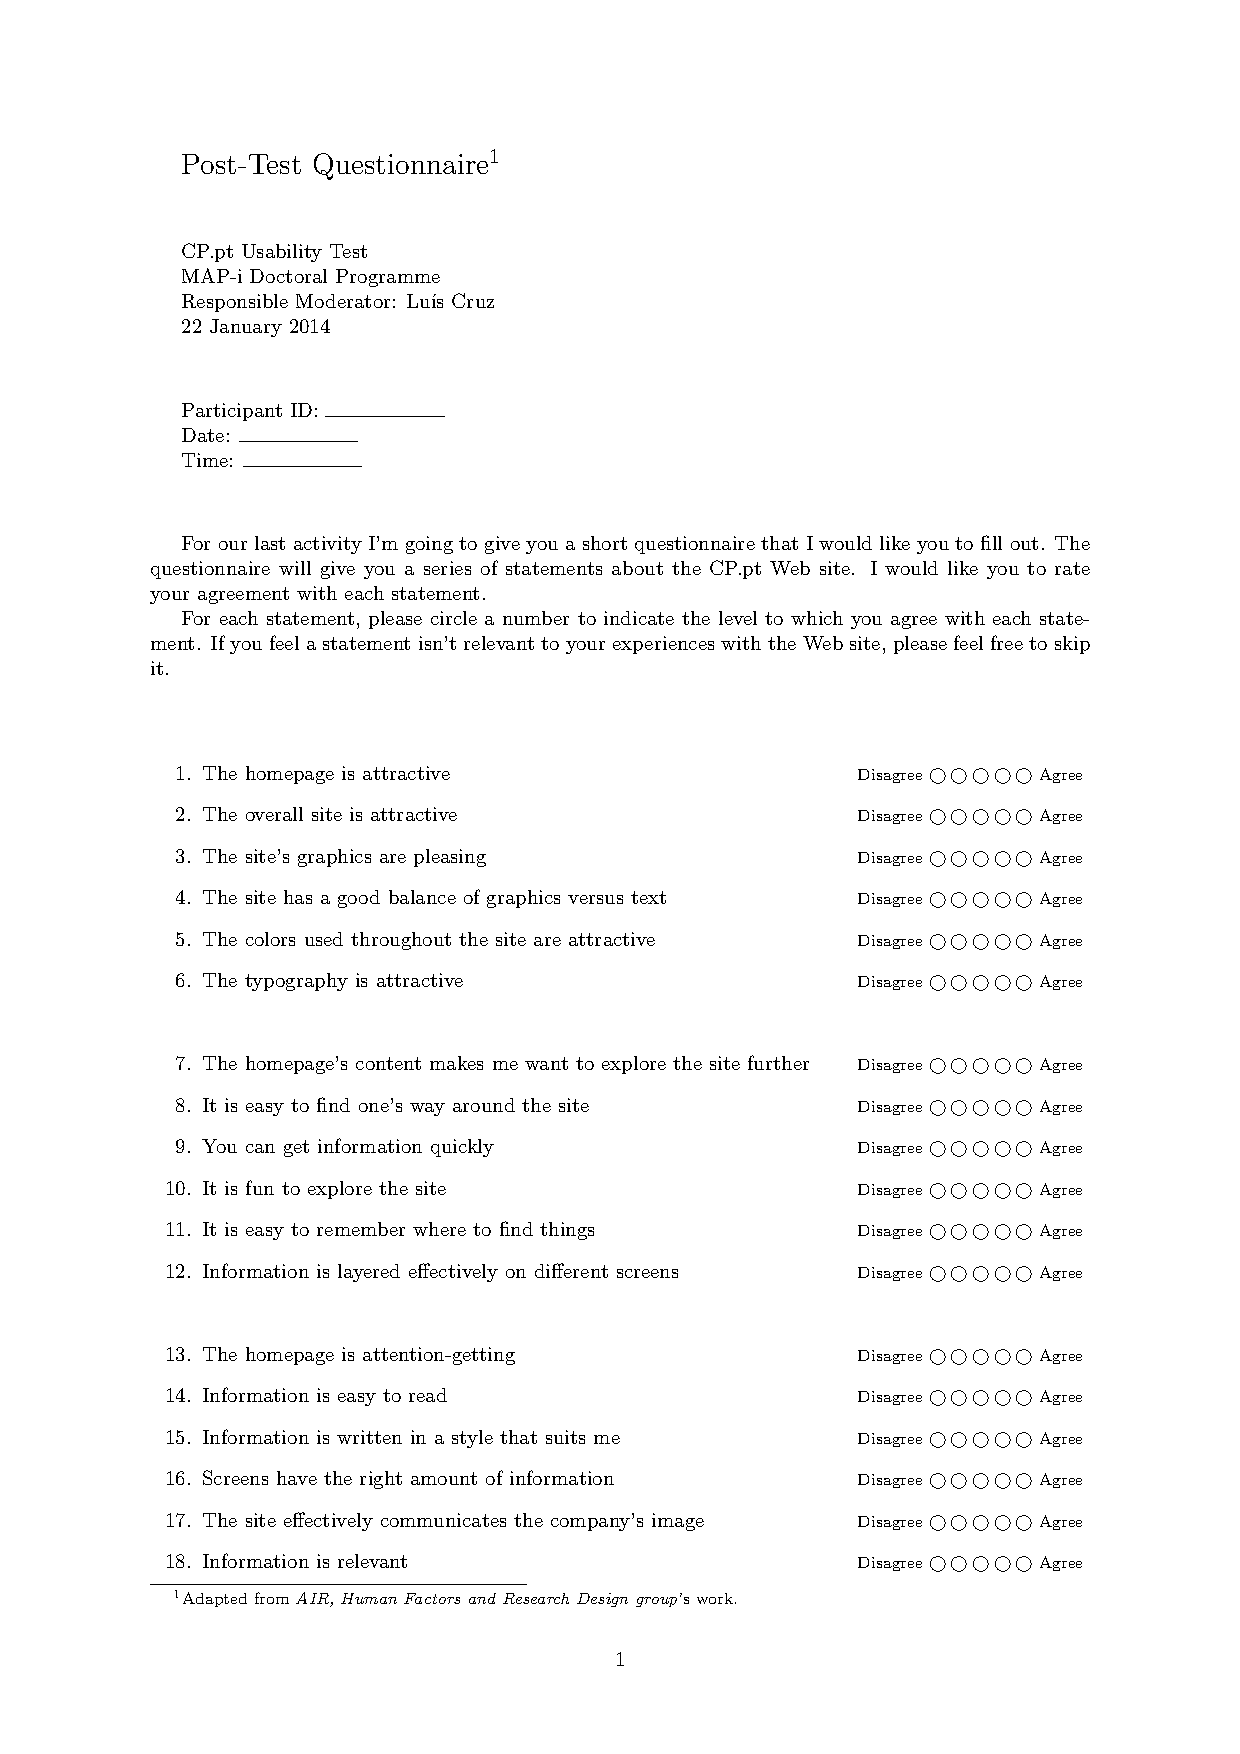
\includepdf[pagecommand=\section{Post-Test Questionnaire}\label{sec:postTestQuestionnaire}\thispagestyle{plain}{The moderator of the usability test observes the behavior of the participant while taking notes in the Data Logging Form. Each task needs one Data Logging Form.}, pages=1, frame=true, scale=0.75, offset=0 -25]{../postTestQuestionnaire/master.pdf}
\includepdf[pagecommand=\thispagestyle{plain}, pages=2-, frame=true, scale=0.75, offset=0 0]{../postTestQuestionnaire/master.pdf}
%----------------------------------------------------------------------------------------
%	BIBLIOGRAPHY
%----------------------------------------------------------------------------------------

\bibliographystyle{apalike}
\bibliography{../bibliography}

%----------------------------------------------------------------------------------------

\end{document}